\documentclass[lithuanian,a4paper,12pt]{article}
\usepackage{babel}
\babelfont{rm}{FreeSerif}
% \usepackage[T1]{fontenc} % Don't need this when using LuaLatex instead of PDFLatex
\usepackage{amsmath}
\usepackage{graphicx}
\usepackage{float}
\usepackage{minted}
\usemintedstyle{vs}
\usepackage{hyperref}
\hypersetup{
    colorlinks=true,
    linkcolor=black,
    urlcolor=cyan,
}
\usepackage{csquotes}
\usepackage{enumitem}
\usepackage{microtype}

\newcommand{\mil}{\mintinline{python}}
\renewcommand{\labelenumii}{\arabic{enumi}.\arabic{enumii}}

\title{Vienmatis optimizavimas}
\author{Kristupas Dansevičius}
\date{\today}

\begin{document}
\maketitle
\tableofcontents

\section{Įvadas}
Šis laboratorinis darbas atsiskaitomas optimizavimo metodų kurse Vilniaus Universitete. 
Šiame darbe nagrinėjami trys vienmačio optimizavimo metodai:
intervalo dalijimo pusiau metodas, auksinio pjūvio metodas ir Niutono metodas. 

\section{Užduotis}
1-ojo laboratorinio darbo (iš viso yra 4 per semestrą) užduoties reikalavimai:
\begin{enumerate}
    \item Suprogramuoti šiuos metodus (naudota Python programavimo kalba)
    \item Aprašyti duotąją \textbf{tikslo funkciją} - tai funkcija, pagal kurią yra optimizuojama naudojant minėtus metodus, t.y., ieškomas jos \textbf{lokalus minimumas}, kuris ir bus ir \textbf{globalusis minimumas}. Taip yra todėl, kad funkcija nurodytam intervale yra \textbf{iškiloji}: tarp bet kurių dviejų funkcijos taškų nubrėžus liniją, visos funkcijos reikšmės yra žemiau šios linijos. Kitaip pasakius, funkcijoje nėra jokių ``duobių'', į kurias optimizuojant galima patekti ir ``užstrigti'', kurios būtų tik lokalūs, bet ne globalūs minimumai. Pagal reikalavimus (pritaikius studento numerio porą skaitmenų), duotoji tikslo funkcija yra:
        \begin{equation*}
            f(x) = \frac{(x^2 - 5)^2}{4}
        \end{equation*}
    \item Minimizuoti funkciją intervalo metodais - intervalo dalijimo pusiau ir auksinio pjūvio - naudojant intervalą $[0,10]$ iki tikslumo $10^{-4}$ bei Niutono metodu nuo $x_0 = 5$ kol žingsnio ilgis (Lipschitzo konstanta / tolerancija) didesnis už $10^{-4}$
    \item Palyginti rezultatus: gauti sprendiniai, rastas funkcijos minimumo įvertis (taško, kuriame funkcija turi mažiausią reikšmę), atliktų žingsnių (iteracijų) ir funkcijų skaičiavimų skaičius (tikslo funkcijos ``iškvietimų'' programoje)
    \item Vizualizuoti tikslo funkciją ir bandymo taškus (kuriuose paskaičiuota tikslo funkcija ir buvo naudojami algoritme)
\end{enumerate}

\section{Tikslo funkcijos aprašymas}
Pateikiamas programoje aprašytos tikslo funkcijos kodas, naudojantis Python objektinio programavimo galimybėmis, panaudojant \mil{class}. Šioje tikslo funkcijos klasės aprašyme yra sekamas tikslo funkcijos iškvietimų kiekis, iškvietimus vykdant iš suprogramuotų optimizavimų metodų kodo. Pasak \url{https://www.sympy.org/scipy-2017-codegen-tutorial/notebooks/22-lambdify.html}, \textquote{Behind the scenes \mil{lambdify} constructs a string representation of the Python code and uses Python's \mil{eval} function to compile the function.} Klasėje yra saugoma simbolinės išraiškos (\url{https://en.wikipedia.org/wiki/S-expression}) ne tik pačios tikslo funkcijos, bet ir jos pirmos ir antros eilės išvestinių (reikalingos su Niutono metodu)

\pagebreak
\begin{minted}{python}
class ObjectiveFunction:
    def __init__(self) -> None:
        self.calls = 0

        self.x: sp.Symbol = sp.symbols('x')
        self.expr: sp.Expr = (self.x**2 - 5)**2 / 4 # type: ignore

        self.expr_prime: sp.Expr = sp.diff(self.expr, self.x)
        self.expr_double_prime: sp.Expr = sp.diff(self.expr, self.x, 2)

        self.f = sp.lambdify(self.x, self.expr, 'numpy')
        self.df = sp.lambdify(self.x, self.expr_prime, 'numpy')
        self.ddf = sp.lambdify(self.x, self.expr_double_prime, 'numpy')

    def __call__(self, x: float) -> float:
        self.calls += 1
        return self.f(x)
    
    def first_derivative(self, x:float) -> float:
        self.calls += 1
        return self.df(x)
    
    def second_derivative(self, x:float) -> float:
        self.calls += 1
        return self.ddf(x)
    
    def print_symbolic(self):
        print("f(x) =", self.expr)
        print("f'(x) =", self.expr_prime)
        print("f''(x) =", self.expr_double_prime)
    
    def reset(self):
        self.calls = 0
\end{minted}

\section{Optimizavimo metodai}
\subsection{Intervalo dalijimo pusiau metodas}
\subsubsection*{Naudojami taškai}
Tai tritaškis intervalo dalijimo pusiau metodas (t.y., kiekvienai optimizavimo algoritmo iteracijai naudojami 3 taškai), kurio principas yra itin paprastas. 
Intervale \mil{[left_bound, right_bound]}, kurio ilgis \mil{interval_length = right_bound - left_bound}, panaudojami 3 taškai:
\begin{itemize}
    \item \mil{x_middle} - vidurinis taškas esantis intervalo viduryje, \\ \mil{x_middle = (left_bound + right_bound) / 2} 
    \item \mil{x1} - tarp kairiojo intervalo krašto \mil{left_bound} ir vidurinio taško \mil{x_middle} esantis taškas, \mil{x1 = left_bound + interval_length / 4}
    \item \mil{x2} - analogiškai kaip \mil{x1}, tik kitoje intervalo pusėje tarp \mil{x_middle} ir \mil{right_bound} esantis taškas, \mil{x2 = right_bound - interval_length / 4}
\end{itemize}
Kiekvienam šių taškų programoje kviečiama tikslo funkcija \mil{f(x)}, kaip tik tą tašką tenka naujai paskaičiuoti ir jis turės prieš tai nebuvusią poziciją intervale. Paskaičiuotos tikslo funkcijos reikšmės taškuose saugomos (ir ``perduodamos'' kitam taškui kai atliekamas vieno taško reiškmės priskyrimas kitam)

\pagebreak
\subsubsection*{Metodo algoritmas}
Algoritmo žingsniai:
\begin{enumerate}
    \item Paskaičiuojami \mil{x_middle}, \mil{interval_length}, \mil{f(x_middle)}
    \item Paskaičiuojami \mil{x1}, \mil{x2}, \mil{f(x1)}, \mil{f(x2)}
    \item Jei \mil{f(x1) < f(x_middle)}, tai:
    \begin{enumerate}
        \item Atmetamas \mil{(x_middle, right_bound]} atliekant keitimą \mil{right_bound = x_middle}
        \item Intervalo centru tampa \mil{x1}, tad atliekamas priskyrimas \mil{x_middle = x1}
        \item Nušokama į 6 punktą
    \end{enumerate}
    \item Jei \mil{f(x2) < f(x_middle)}, tai:
    \begin{enumerate}
        \item Atmetamas \mil{[left_bound, x_middle)} analogiškai keičiant \mil{left_bound = x_middle}
        \item Intervalo centru tampa \mil{x2}, tad atliekamas priskyrimas \mil{x_middle = x2}
        \item Nušokama į 6 punktą
    \end{enumerate}
    \item Jei prieinamas paskutinis atvejis, t.y., atliekamoje iteracijoje mažiausia tikslo funkcijos reikšmė turima su intervalo centru \mil{x_middle}: 
    \begin{enumerate}
        \item Intervalo centru \mil{x_middle} ir lieka, atmetama po 0.25 intervalo nuo abiejų kraštų. Reiškia, atmetami intervalai \mil{[left_bound, x1)} ir \mil{(x2, right_bound]} atliekant priskyrimus \mil{left_bound = x1} ir \mil{right_bound = x2}
    \end{enumerate}
    \item Skaičiuojamas \mil{interval_length}, kuris, jei yra pakankamai mažas (mažesnis už 
    $\epsilon$, t.y., nurodytą tikslumą, kode įvardintą kaip \mil{tolerance_lipschitz_constant}, kuris darbe nurodytas būti $10^{-4}$, skaičiavimai baigiami, o jei ne - einama į 2 punktą. 
\end{enumerate}

Suprogramuotam metode einamoje iteracijoje \mil{x2} ir \mil{f(x2)} neskaičiuojami, kai 3-ame punkte tikrinimo sąlyga grąžina tiesą

\pagebreak
\subsubsection*{Programinis kodas}
Šio metodo įgyvendinimas programiniam kode čia pateikiamas ``suprastinamas'', be kodo eilučių darančių tarpinių metodo iteracijų reikšmių spausdinimą

\begin{minted}{python}
def bisection_method(
        objective_function: ObjectiveFunction, 
        interval: tuple[int, int] = (0, 10), 
        tolerance_lipschitz_constant: float = 10**-4
        ) -> OptimizationResult:
    
    # Points kept for plotting later
    x_min: float
    xs: list[float] = []
    
    left_bound: float = interval[0]
    right_bound: float = interval[1]
    interval_length: float = right_bound - left_bound

    objective_function.reset()
    f = objective_function.__call__

    x_middle: float = (left_bound + right_bound) / 2 # 1.
    x1: float | None = None
    x2: float | None = None
    f_x_middle: float = f(x_middle) # 1.
    f_x1: float | None = None
    f_x2: float | None = None

    iteration: int = 0
    while interval_length > tolerance_lipschitz_constant: # 6
        interval_length = right_bound - left_bound
            
        x1 = left_bound + interval_length / 4 # 2.
        f_x1 = f(x1) # 2.

        xs.append(x1)
        xs.append(x_middle)
        
        if f_x1 < f_x_middle: # 3. x_middle becomes x1
            right_bound = x_middle # 3.1
            x_middle = x1 # 3.2
            f_x_middle = f_x1 # 3.2
            interval_length = right_bound - left_bound
            iteration += 1
            continue # 6. is while loop condition

        else: # 2.
            x2 = right_bound - interval_length / 4 # 2.
            f_x2 = f(x2) # 2.
            xs.append(x2)
            if f_x2 < f_x_middle: # 4. x_middle becomes x2
                left_bound = x_middle # 4.1 
                x_middle = x2 # 4.2 
                f_x_middle = x2 # 4.2
            else: # 5. x_middle stays x_middle
                x_middle = x_middle
                left_bound = x1 # 5.1 
                right_bound = x2 # 5.1

        interval_length = right_bound - left_bound
        iteration += 1
    # Loop end
    x_min: float = (left_bound + right_bound) / 2
    return OptimizationResult(
        x_min=x_min, 
        xs=xs, 
        iterations=iteration, 
        function_calls=objective_function.calls
    )
\end{minted}

\pagebreak
\subsection{Auksinio pjūvio metodas}
\subsubsection*{Naudojami taškai}
Šis metodas yra dvitaškis intervalo dalijimo metodas (bet ne pusiau, su viena iteracija atmetama mažesnė intervalo dalis nei su intervalo dalijimo pusiau metodu). Intervale \mil{[left_bound, right_bound]}, kurio ilgis \mil{interval_length = right_bound - left_bound}, kiekvienai iteracijai naudojami tik 2 taškai, \mil{x1} ir \mil{x2}. $\tau$ (\mil{tau}) yra teigiamas Fibonačio skaičius $\tau = 0.61803\ldots$, gaunamas iš lygybės
\begin{equation*}
    \frac{1 - \tau}{1} = \frac{\tau - (1 - \tau)}{\tau}
\end{equation*}
, iš kurios išplaukia
\begin{equation*}
    \tau = (-1 \pm \sqrt{5}) / 2
\end{equation*}

\pagebreak
\subsubsection*{Metodo algoritmas}
Algoritmo žingsniai:
\begin{enumerate}
    \item Paskaičiuojamas intervalo ilgis \mil{interval_length = right_bound - left_bound}, taškai
    \begin{minted}{python}
        x1 = right_bound - tau * interval_length 
        x2 = left_bound + tau * interval
    \end{minted}
    Paskaičiuojama \mil{f(x1)} ir \mil{f(x2)}
    \item Jei \mil{f(x2) < f(x1)}:
    \begin{enumerate}
        \item Atmetama intervalo dalis \mil{[left_bound, x1)} priskiriant \mil{left_bound = x1}, perskaičiuojamas \mil{interval_length}
        \item \mil{x1 = x2} (Kairiuoju tašku \mil{x1} tampa anksčiau buvęs dešinysis taškas \mil{x2})
        \item Naujasis dešinysis taškas \mil{x2 = left_bound + tau * interval_length}, apskaičiuojamas \mil{f(x2)}
    \end{enumerate}
    \item Kitu atveju:
    \begin{enumerate}
        \item Atmetama intervalo dalis \mil{(x2, right_bound]} priskiriant \mil{right_bound = x2},
        perskaičiuojamas \mil{interval_length}
        \item \mil{x2 = x1} (Dešiniuoju tašku \mil{x2} tampa anksčiau buvęs kairysis taškas \mil{x1}) 
        \item Naujasis kairysis taškas \mil{x1 = right_bound - tau * interval_length}, apskaičiuojamas \mil{f(x1)}
    \item Jei \mil{interval_length} yra pakankamai mažas (mažesnis už $\epsilon$, t.y., nurodytą tikslumą, kode įvardintą kaip \mil{tolerance_lipschitz_constant}, kuris darbe nurodytas būti $10^{-4}$, skaičiavimai baigiami, o jei ne - einama į 2 punktą. 
    \end{enumerate}
\end{enumerate}

\pagebreak
\subsubsection*{Programinis kodas}
Šio metodo įgyvendinimas programiniam kode čia pateikiamas ``suprastinamas'', be kodo eilučių darančių tarpinių metodo iteracijų reikšmių spausdinimą

\begin{minted}{python}
    def golden_section_method(
        objective_function: ObjectiveFunction, 
        interval: tuple[int, int] = (0, 10), 
        tolerance_lipschitz_constant: float = 10**-4
        ) -> OptimizationResult:
    
    objective_function.reset()
    f = objective_function.__call__
    left_bound: float 
    right_bound: float 
    left_bound, right_bound = interval
    interval_length: float = right_bound - left_bound # 1.
    
    tau: float = (-1 + sqrt(5)) / 2
    x1: float = right_bound - tau * interval_length # 1.
    x2: float = left_bound + tau * interval_length # 1.
    f_x1: float = f(x1) # 1.
    f_x2: float = f(x2) # 1.

    # Points kept for plotting later
    xs: list[float] = [x1, x2]
    
    iteration: int = 0
    while interval_length > tolerance_lipschitz_constant:
        print("Current iteration:", iteration)
        print("Interval:", [left_bound, right_bound])
        print("Interval length:", interval_length)
        print()
        
        if f_x2 < f_x1: # 2.
            left_bound = x1 # 2.1 remove interval [left_bound; x1)
            interval_length = right_bound - left_bound # 2.1 / 3.1
            x1 = x2 # 2.2
            f_x1 = f_x2
            x2 = left_bound + tau * interval_length # 2.3
            f_x2 = f(x2) # 2.3
            xs.append(x2)
        else: # 3.
            right_bound = x2 # 3.1 remove interval (x2; right_bound]
            interval_length = right_bound - left_bound # 2.1 / 3.1
            x2 = x1 # 3.2
            f_x2 = f_x1
            x1 = right_bound - tau * interval_length # 3.3
            f_x1 = f(x1) # 3.3
            xs.append(x1)
            
        iteration += 1
        
    x_min: float = (left_bound + right_bound) / 2
    return OptimizationResult(
        x_min=x_min, 
        xs=xs, 
        iterations=iteration, 
        function_calls=objective_function.calls
    )
\end{minted}
\pagebreak

\subsection{Niutono metodas}


\section{Rezultatai}
Gauti šie rezultatai:
\begin{itemize}
    \item Intervalo dalijimo pusiau metodas: 
        $x_{\min} \approx 2.236$, iteracijų: 17, funkcijos iškvietimų: 28
    \item Auksinio pjūvio metodas:
        $x_{\min} \approx 2.236$, iteracijų: 24, funkcijos iškvietimų: 26
    \item Niutono metodas:
        $x_{\min} \approx 2.236$, iteracijų: 6, funkcijos iškvietimų: 12
\end{itemize}

\section{Vizualizacija}
Žemiau pateikiamos tikslo funkcijos ir taikytų metodų vizualizacijos.
\begin{figure}[H]
    \centering
    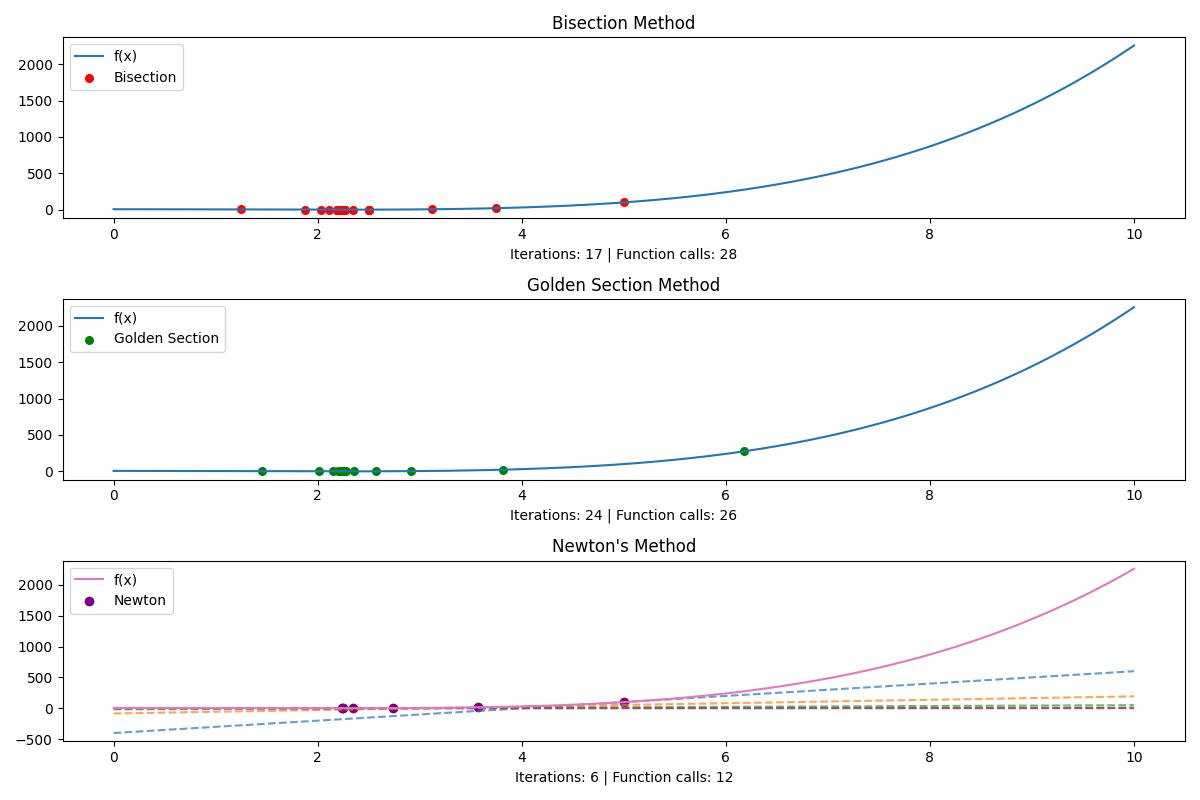
\includegraphics[width=\textwidth,height=10cm]{figure-1.jpeg}
    \caption{\label{fig:all}Funkcijos $f(x)$ optimizavimo vizualizacija.}
\end{figure}

\section{Išvados}
\begin{itemize}
    \item Visi metodai rado minimumą ties $x \approx \sqrt{5}$.
    \item Intervalo metodai (intervalo dalijimo pusiau ir auksinio pjūvio) reikalauja daugiau iteracijų ir tikslo funkcijos iškvietimų, bet yra paprastesni.
\end{itemize}

\pagebreak
\section{Kodas}
\inputminted{python}{../code/main.py}
\pagebreak

\section{Šaltiniai}
\begin{enumerate}
    \item Python paketo \mintinline{python}{sympy} oficialaus puslapio 2017-ųjų metų užrašų tipo mokymo programa / tutorial: \url{https://www.sympy.org/scipy-2017-codegen-tutorial/notebooks/22-lambdify.html}
    \item Simbolinių išraiškų Wikipedia šaltinis:\url{https://en.wikipedia.org/wiki/S-expression}
    \item Paskaitų skaidrės: ``moodle'' sistemoje pateiktos dėstytojo J. Žilinsko paskaitų skaidrės
\end{enumerate}

\end{document}